\subsection{Behavior of GPU memory access performance}  \label{GPUBehavior}

GPU vendors do not disclose much information on the micro-architecture of their GPUs.
Hence, in order to optimize GPGPU programs so that they can more efficiently exploit hardware
resources, it is often necessary to reverse engineer the performance behavior of the GPUs through
experimentation.
In this section, we present the results of some of the experiments we ran to gain more insight into the memory subsystem.
All results we present here were obtained on an Nvidia GTX~Titan~Black.

%\todo{Don't you think we should cut the rest of this par, cause we already mentioned these parameters earlier in this section, and just say "All results we present were obtained on the Nvidia GTX 680.}
%All
%experiments were run on the NVIDIA GeForce GTX 680, with 1,536 cores in 8 SMXs. All SMXs are
%onnected to a 512KB of L2 cache and 2GB of DRAM. Each SMX can host up to 2,048 threads at the
%same time.

\subsubsection{Memory access throughput}
In our first set of experiments, we used a micro-benchmark that has threads read disjoint (non-contiguous) subsets of data
located in the L2 cache as quickly as possible.
The benchmark is parameterized so that the degree of coalescing can be varied.
Figure~\ref{fig:MemBandwidth} shows the maximum L2 memory bandwidth obtained, measured as
the number of bytes transferred over the network, when servicing 4-way coalesced
accesses from the L2 cache as the number of threads running in each thread block is increased up to
1,024.

%\footnote{
%	4-way coalesced means that four data items, accessed by simultaneous threads, 
%	lie within a 128 byte segment.} 


\begin{figure}
\center
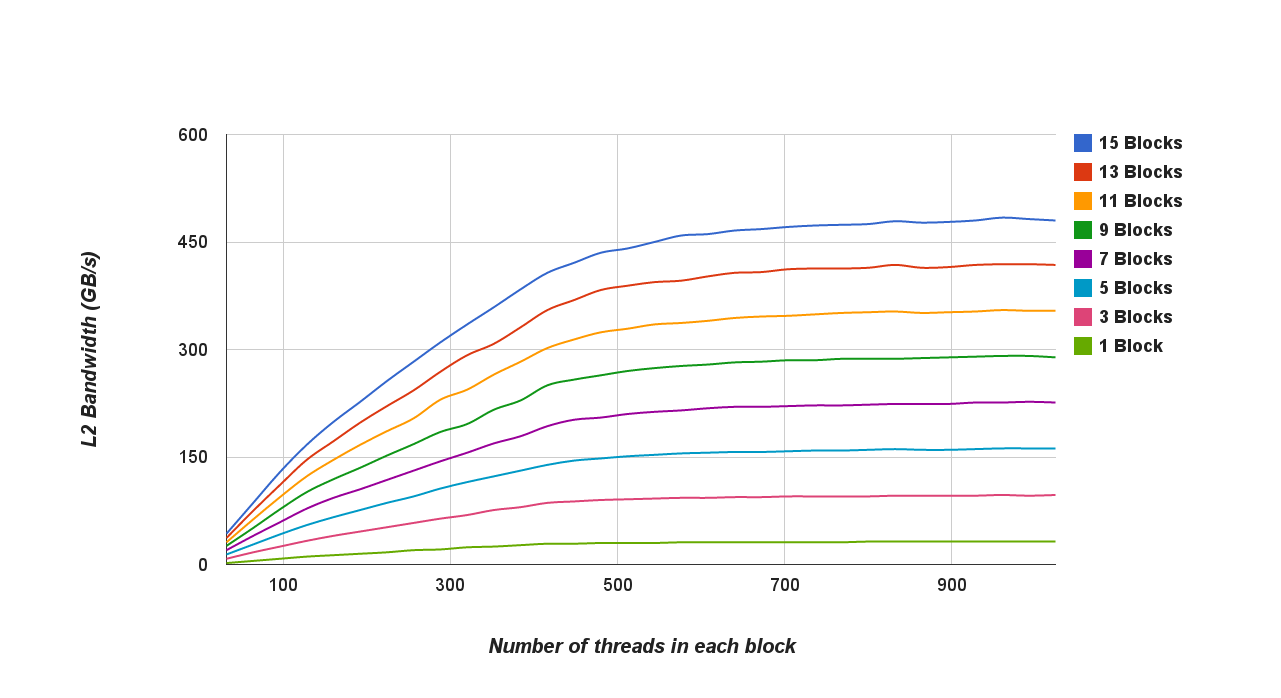
\includegraphics[scale=0.21]{AllInL2MultipleSM4WayColaesced.png}
\caption{\footnotesize\textnormal{L2 memory throughput as a function of number of threads in a thread block. Each curve represents the throughput for a different number of thread blocks (1 to 15) with each thread block running 1,024 threads.}}
\label{fig:MemBandwidth}
\vspace{-0.3cm}
\end{figure}

% \begin{figure}
% 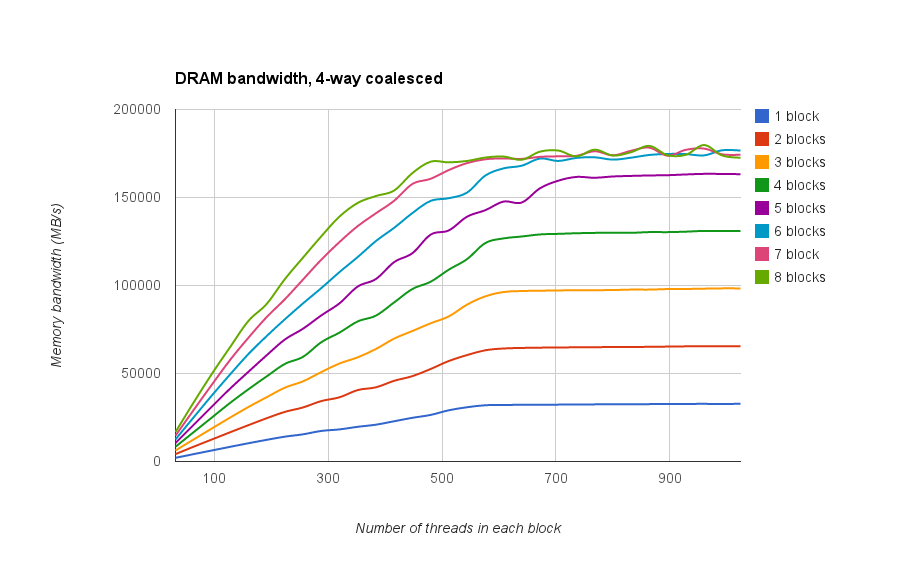
\includegraphics[width=\linewidth]{DRAMBandwidth4-wayCoalesced.png}
% \caption{DRAM memory throughput as a function of number of threads in a thread block for $n=1..8$
% thread-blocks}
% \label{fig:DRAMBandwidth}
% \end{figure}


Each curve represents a different number of thread blocks used, and each block uses the same number of threads.
The thread blocks are assigned to SMXs in a round robin manner by the hardware.
Focusing on the bottom curve, representing an experiment that has just one thread block running on
one SMX, one can see that the memory throughput flattens out after about 512 threads at slightly less
than 32~GB/s.\footnote{
    Our experiments show that varying the degree of coalescing does not completely
    remove the flattening out behavior. 
    However, the smaller the coalescing degree (e.g. 1-way coalesced), the
    earlier the curve flattens out.}
We observe similar behavior for DRAM (not shown) when we adjusted the micro-benchmarks to only access data certain to not be in the L2 cache, except that the throughput flattens out
earlier at about 480 threads, reaching to a peak bandwidth of 307~GB/s with 15 blocks.
%\todo{fill in the XX and YY above}
% shown in Figure~\ref{fig:DRAMBandwidth}.


It is difficult to assess what causes the stagnation in L2 and DRAM throughput.
However the near-linear scalability with the number of thread blocks indicates that the bottleneck
is in the interconnect or in the SMX itself (e.g., coalescing units) rather than L2 or DRAM.
This is shown in Figure~\ref{fig:L2-DRAM-bandwidth} where we show the throughput as a function of
the number of thread blocks with each thread block running 1,024 threads.
Each point along the L2 bandwidth curve is equal to the end point (at 1,024 threads) of the corresponding curve of
Figure~\ref{fig:MemBandwidth}.
L2 throughput increases almost linearly, reaching close to 480~GB/s with 15 blocks. DRAM throughput increases
almost linearly up to 10 thread blocks at which point the bandwidth limits at around 300GB/s.

\begin{figure}
\vspace{-0.8cm}
\center
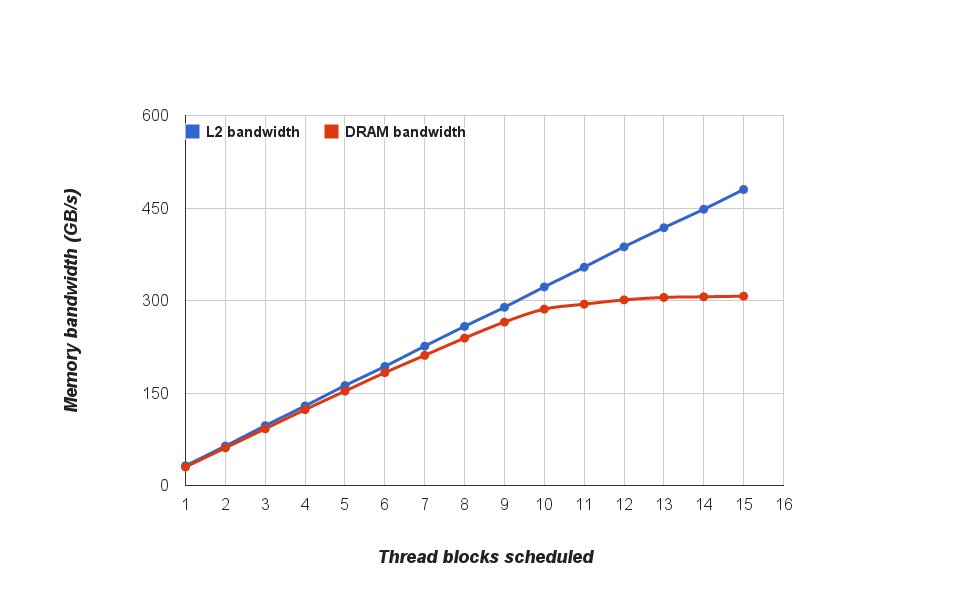
\includegraphics[scale=0.3]{DRAML2Bandwidth-4wayCoalesced.png}
\caption{\footnotesize\textnormal{L2 and DRAM memory bandwidth as a function of number of thread blocks where each thread
block is running 1,024 threads and the memory accesses are 4-way coalesced.
%\todo{replace figure withone for 4-way coalesced} 
}}
\label{fig:L2-DRAM-bandwidth}
\vspace{-0.3cm}
\end{figure}

The above results measured the amount of data transferred to the SMXs by the
hardware.
In practice, however, much of this data may not actually be used by the
application.
For example, for non-coalesced accesses, each 4-byte integer access will result in 32
byte transfer, of which only 4 are actual used.

The end result is that the memory access latencies actually experienced in
practice will be far larger than the theoretical access latencies presented in
Section~\ref{GPUBackground}.
This implies that an SMX-local L1 cache, whether implemented in hardware or software, can
dramatically reduce the average latency of accesses with locality, if implemented appropriately.
In particular, in contrast to L2 and DRAM throughput,  shared memory throughput within an SMX (not shown) does not flatten out and reaches 60GB/s (for an aggregate throughput of close to 900GB/s with 15 SMXs).
%\todo{Not sure... I don't find the order bad...:  The order of sentences of this parag needs to be changed. First starting by saying that shared memory
%curves do not flatten out (preferably showing the figure, if space permits), and then saying that
%therefore, if L1 is implemented properly, it could be highly beneficial.}








